\documentclass[tikz, border=10pt]{standalone}

\usepackage{tikz}
\usetikzlibrary{snakes}

\tikzset{
    every node/.style = {minimum size=1cm},
    level/.style = {sibling distance=60mm/#1}
}

\begin{document}
    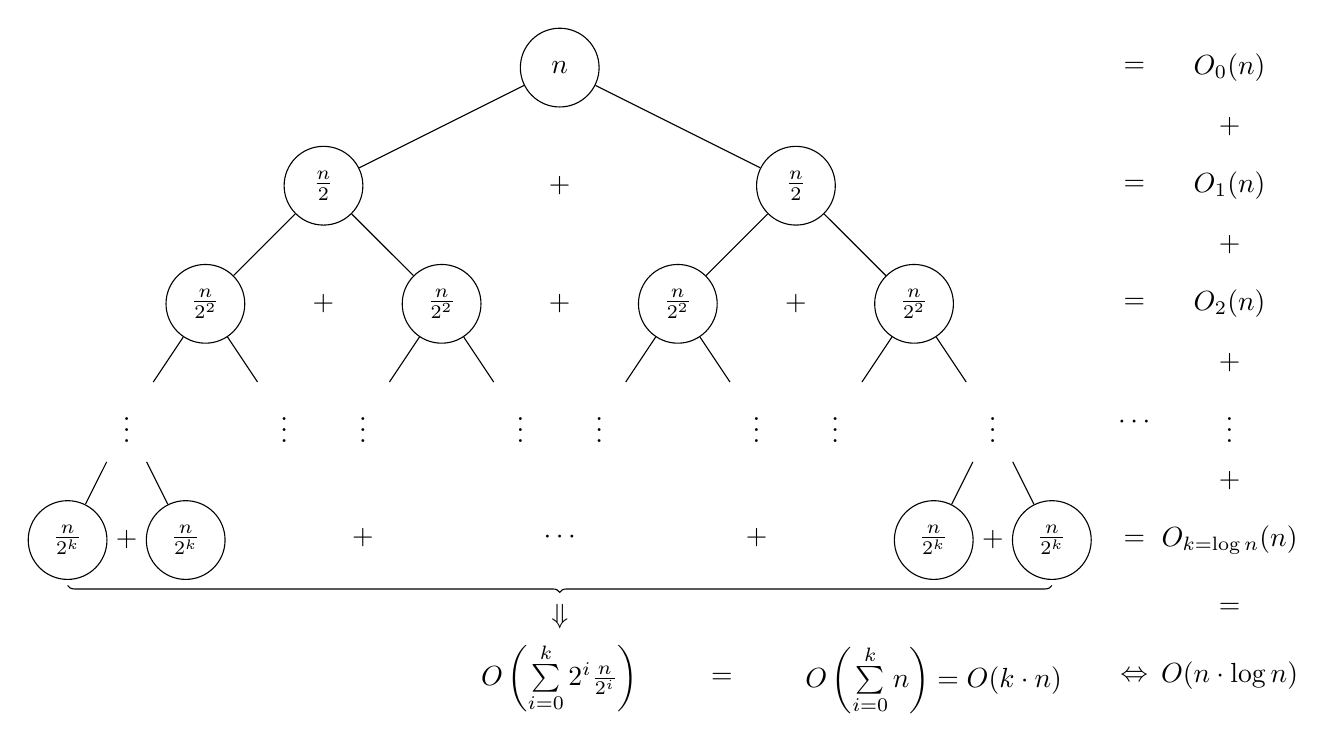
\begin{tikzpicture}
        \node[circle, draw] (r) {$n$}
            child {node[circle, draw] {$\frac{n}{2}$}
                child {node[circle, draw] {$\frac{n}{2^2}$}
                    child {node {$\vdots$}
                        child {node[circle, draw] {$\frac{n}{2^k}$}}
                        child {node[circle, draw] {$\frac{n}{2^k}$}}
                    }
                    child {node {$\vdots$}}
                }
                child {node[circle, draw] {$\frac{n}{2^2}$}
                    child {node {$\vdots$}}
                    child {node {$\vdots$}}
                }
            }
            child {node[circle, draw] {$\frac{n}{2}$}
                child {node[circle, draw] {$\frac{n}{2^2}$}
                    child {node {$\vdots$}}
                    child {node {$\vdots$}}
                }
                child {node[circle, draw] {$\frac{n}{2^2}$}
                    child {node {$\vdots$}}
                    child {node {$\vdots$}
                        child {node[circle, draw] {$\frac{n}{2^k}$}}
                        child {node[circle, draw] {$\frac{n}{2^k}$}}
                    }
                }
            };
            
        \begin{scope}[shift={([xshift=8cm]r.east)}]
            \tikzset{
                edge from parent/.style = {draw=none},
                grow=down
            }
            \node (t) {$O_0(n)$}
                child {node {$O_1(n)$}
                    child {node {$O_2(n)$}
                        child {node {$\vdots$}
                            child {node {$O_{k = \log{n}}(n)$}
                                child {node[below=-8pt] {$O(n\cdot\log{n})$}}
                            }
                        }    
                    }
                };
        \end{scope}    
        
        \path (r-1) -- node {$+$} (r-2);
        \path (r-1-1) -- node {$+$} (r-1-2);
        \path (r-1-2) -- node {$+$} (r-2-1);
        \path (r-2-1) -- node {$+$} (r-2-2);
        \path (r-1-1-1-1) -- node {$+$} (r-1-1-1-2);
        \path (r-2-2-2-1) -- node {$+$} (r-2-2-2-2);
        \path (r-1-2-1.south) node[below=13pt] {$+$} -- node (above eq1) [below=13pt] {$\cdots$} (r-2-1-2.south) node[below=13pt] {$+$};
        \path[draw, snake=brace, mirror snake, raise snake=2pt] (r-1-1-1-1.south) -- (r-2-2-2-2.south);
        \path (above eq1.south) node [below=20pt] (eq1) {$O\left(\sum\limits_{i=0}^{k}2^i\frac{n}{2^i}\right)$};
        \path (above eq1) -- (eq1) node[pos=0.7] {$\Downarrow$};
        \path (r-2-2-2-1.south) node[below=20pt] (eq2) {$O\left(\sum\limits_{i=0}^{k}n\right) = O(k\cdot n)$};
        \path (eq1) -- node {$=$} (eq2);
        
        \path (t) -- node {$+$} (t-1) -- node {$+$} (t-1-1) -- node {$+$} (t-1-1-1) -- node {$+$} (t-1-1-1-1) -- node {$=$} (t-1-1-1-1-1);
        \path (t) node[left=20pt] {$=$}
              (t-1) node[left=20pt] {$=$}
              (t-1-1) node[left=20pt] {$=$}
              (t-1-1-1) node[left=20pt] {$\cdots$}
              (t-1-1-1-1) node[left=20pt] {$=$}
              (t-1-1-1-1-1) node[left=20pt] {$\Leftrightarrow$};
    \end{tikzpicture}
\end{document}